% This is "sig-alternate.tex" V2.1 April 2013
% This file should be compiled with V2.5 of "sig-alternate.cls" May 2012
%
% This example file demonstrates the use of the 'sig-alternate.cls'
% V2.5 LaTeX2e document class file. It is for those submitting
% articles to ACM Conference Proceedings WHO DO NOT WISH TO
% STRICTLY ADHERE TO THE SIGS (PUBS-BOARD-ENDORSED) STYLE.
% The 'sig-alternate.cls' file will produce a similar-looking,
% albeit, 'tighter' paper resulting in, invariably, fewer pages.
%
% ----------------------------------------------------------------------------------------------------------------
% This .tex file (and associated .cls V2.5) produces:
%       1) The Permission Statement
%       2) The Conference (location) Info information
%       3) The Copyright Line with ACM data
%       4) NO page numbers
%
% as against the acm_proc_article-sp.cls file which
% DOES NOT produce 1) thru' 3) above.
%
% Using 'sig-alternate.cls' you have control, however, from within
% the source .tex file, over both the CopyrightYear
% (defaulted to 200X) and the ACM Copyright Data
% (defaulted to X-XXXXX-XX-X/XX/XX).
% e.g.
% \CopyrightYear{2007} will cause 2007 to appear in the copyright line.
% \crdata{0-12345-67-8/90/12} will cause 0-12345-67-8/90/12 to appear in the copyright line.
%
% ---------------------------------------------------------------------------------------------------------------
% This .tex source is an example which *does* use
% the .bib file (from which the .bbl file % is produced).
% REMEMBER HOWEVER: After having produced the .bbl file,
% and prior to final submission, you *NEED* to 'insert'
% your .bbl file into your source .tex file so as to provide
% ONE 'self-contained' source file.
%
% ================= IF YOU HAVE QUESTIONS =======================
% Questions regarding the SIGS styles, SIGS policies and
% procedures, Conferences etc. should be sent to
% Adrienne Griscti (griscti@acm.org)
%
% Technical questions _only_ to
% Gerald Murray (murray@hq.acm.org)
% ===============================================================
%
% For tracking purposes - this is V2.0 - May 2012

\documentclass{sig-alternate-05-2015}
%\g@addto@macro{\UrlBreaks}{\UrlOrds}
%\usepackage{hyperref}


\begin{document}

% Copyright
\setcopyright{acmcopyright}
%\setcopyright{acmlicensed}
%\setcopyright{rightsretained}
%\setcopyright{usgov}
%\setcopyright{usgovmixed}
%\setcopyright{cagov}
%\setcopyright{cagovmixed}


% DOI
\doi{http://dx.doi.org/10.1145/2987538.2987546}

% ISBN
\isbn{978-1-4503-4801-0/16/09}

%Conference
\conferenceinfo{RecSys Challenge '16, }{September 15 2016, Boston, MA, USA}

\acmPrice{\$15.00}

%
% --- Author Metadata here ---
%\conferenceinfo{RecSys}{'16 Boston, MA USA}
\CopyrightYear{2016} % Allows default copyright year (20XX) to be over-ridden - IF NEED BE.
%\crdata{0-12345-67-8/90/01}  % Allows default copyright data (0-89791-88-6/97/05) to be over-ridden - IF NEED BE.
% --- End of Author Metadata ---

\title{A Bottom-Up Approach to Job Recommendation System}
%\subtitle{[Extended Abstract]
%\titlenote{A full version of this paper is available as
%\textit{Author's Guide to Preparing ACM SIG Proceedings Using
%\LaTeX$2_\epsilon$\ and BibTeX} at
%\texttt{www.acm.org/eaddress.htm}}}
%
% You need the command \numberofauthors to handle the 'placement
% and alignment' of the authors beneath the title.
%
% For aesthetic reasons, we recommend 'three authors at a time'
% i.e. three 'name/affiliation blocks' be placed beneath the title.
%
% NOTE: You are NOT restricted in how many 'rows' of
% "name/affiliations" may appear. We just ask that you restrict
% the number of 'columns' to three.
%
% Because of the available 'opening page real-estate'
% we ask you to refrain from putting more than six authors
% (two rows with three columns) beneath the article title.
% More than six makes the first-page appear very cluttered indeed.
%
% Use the \alignauthor commands to handle the names
% and affiliations for an 'aesthetic maximum' of six authors.
% Add names, affiliations, addresses for
% the seventh etc. author(s) as the argument for the
% \additionalauthors command.
% These 'additional authors' will be output/set for you
% without further effort on your part as the last section in
% the body of your article BEFORE References or any Appendices.

\numberofauthors{2} %  in this sample file, there are a *total*
% of EIGHT authors. SIX appear on the 'first-page' (for formatting
% reasons) and the remaining two appear in the \additionalauthors section.
%
\author{
% You can go ahead and credit any number of authors here,
% e.g. one 'row of three' or two rows (consisting of one row of three
% and a second row of one, two or three).
%
% The command \alignauthor (no curly braces needed) should
% precede each author name, affiliation/snail-mail address and
% e-mail address. Additionally, tag each line of
% affiliation/address with \affaddr, and tag the
% e-mail address with \email.
%
% 1st. author
\alignauthor
Sonu K. Mishra\\
       \affaddr{Computer Science Department}\\
       \affaddr{University of California Los Angeles}\\
       \affaddr{California, U.S.A}\\
       \email{skmishra@cs.ucla.edu}
% 2nd. author
\alignauthor
Manoj Reddy\titlenote{Both authors contributed equally}\\
       \affaddr{Computer Science Department}\\
       \affaddr{University of California Los Angeles}\\
       \affaddr{California, U.S.A}\\
       \email{mdareddy@cs.ucla.edu}
}


\maketitle
\begin{abstract}
Recommendation Systems are omnipresent on the web nowadays. Most websites today are striving to provide quality recommendations to their customers in order to increase and retain their customers. In this paper, we present our approaches to design a job recommendation system for a career based social networking website -- XING. We take a bottom up approach: we start with deeply understanding and exploring the data and gradually build the smaller bits of the system. We also consider traditional approaches of recommendation systems like collaborative filtering and discuss its performance. The best model that we produced is based on Gradient Boosting algorithm. Our experiments show the efficacy of our approaches. This work is based on a challenge organized by ACM RecSys conference 2016. We achieved a final full score of \textbf{1,411,119.11} with \textbf{rank 20} on the official leader board.
\end{abstract}


%
% The code below should be generated by the tool at
% http://dl.acm.org/ccs.cfm
% Please copy and paste the code instead of the example below.
%

\begin{CCSXML}
<ccs2012>
<concept>
<concept_id>10002951.10003317.10003347.10003350</concept_id>
<concept_desc>Information systems~Recommender systems</concept_desc>
<concept_significance>500</concept_significance>
</concept>
<concept>
<concept_id>10010147.10010257.10010321.10010333</concept_id>
<concept_desc>Computing methodologies~Ensemble methods</concept_desc>
<concept_significance>300</concept_significance>
</concept>
</ccs2012>
\end{CCSXML}
\sloppy
{
\ccsdesc[500]{Information systems~Recommender systems}
\ccsdesc[300]{Computing methodologies~Ensemble methods}
}

%\begin{CCSXML}
%<ccs2012>
% <concept>
%  <concept_id>10010520.10010553.10010562</concept_id>
%  <concept_desc>Computer systems organization~Embedded systems</concept_desc>
%  <concept_significance>500</concept_significance>
% </concept>
% <concept>
%  <concept_id>10010520.10010575.10010755</concept_id>
%  <concept_desc>Computer systems organization~Redundancy</concept_desc>
%  <concept_significance>300</concept_significance>
% </concept>
% <concept>
%  <concept_id>10010520.10010553.10010554</concept_id>
%  <concept_desc>Computer systems organization~Robotics</concept_desc>
%  <concept_significance>100</concept_significance>
% </concept>
% <concept>
%  <concept_id>10003033.10003083.10003095</concept_id>
%  <concept_desc>Networks~Network reliability</concept_desc>
%  <concept_significance>100</concept_significance>
% </concept>
%</ccs2012>
%\end{CCSXML}
%
%\ccsdesc[500]{Computer systems organization~Embedded systems}
%\ccsdesc[300]{Computer systems organization~Redundancy}
%\ccsdesc{Computer systems organization~Robotics}
%\ccsdesc[100]{Networks~Network reliability}


%
% End generated code
%

%
%  Use this command to print the description
%
\printccsdesc

% We no longer use \terms command
%\terms{Theory}

\keywords{Recommendation System; Collaborative Filtering; Regression; Gradient Boosting}

\section{Introduction}
Rapid advancements in computer technology have led to the tremendous amount of user data. With the increase in magnitude of data, the requirements and expectations of users have also increased. Major companies around the world have grabbed the opportunity and have started using data to predict the behavior and needs of their customers, and provide their recommendations accordingly. This has led to increased customer satisfaction, and this quickly transformed into multi-fold profit increase for companies. Consequently, recommendation systems are everywhere on web. Online shopping websites like Amazon, Flipkart, and Alibaba recommend products, friendship social networking websites like Facebook and Google+ recommend friends, professional networking website like LinkedIn and XING recommend jobs, travel websites recommend various travel and accommodation offers, and so on.

In this paper, we present our work on developing a job recommendation system for XING. The work is a part of a competition floated by ACM RecSys 2016 [1]. We believe the design of any good system is solely based on how deeply the developers understand the system and the data. We therefore take a bottom-up approach in which we first deal with each dataset individually and analyze how each of them can help in providing quality recommendations to users. Once we are equipped with a deeper insight into data, we combine the individual components to build a very powerful recommendation system. We also consider traditional approaches like collaborative filtering (CF) [3] and discuss how we can use those to improve our system.

The rest of the paper is organized as follows. In Section $2$ we present the datasets that are used to build the system. In Section $3$, we present the various approaches that we considered while building the recommendation system. In Section $4$, we study the performance and discuss pros and cons of these approaches. Finally, we conclude the paper and briefly discuss our future work in Section $5$.

\section{Datasets}
There are four datasets provided by the competition in addition to a list of $150K$ target users. For each target user, we have to generate up to $30$ recommendations. Here we provide the brief description of the datasets. More detailed information is available at [2].

\subsection{Users}
This dataset contains information obtained from the users profiles. The fields provided are: user ID, job roles, career level, discipline, industry, various fields for work experience, region, country, education, etc. There are $1.5M$ entries in this file.

\subsection{Items}
This dataset contains information about the job items that have been posted on the website. The fields provided are: item ID, job roles, discipline, industry, type of employment, location, etc. There are $1.3M$ entries in this file.

\subsection{Impressions}
This dataset contains information about what items were shown to the users on XING, using the existing recommender system. The fields provided are: user ID, year, week and item IDs. There are $10M$ entries in this file

\subsection{Interactions}
The interactions file contains information about the actions performed by users on various job items. The fields provided are: user ID, item ID, interaction type and timestamp. There are $8M$ entries in this file. The interaction type consists of the following values:
\begin{enumerate}
  \item the user clicked on the item
  \item the user bookmarked the item on XING
  \item the user clicked on the application form button
  \item the user deleted the recommendation (clicking on ``x")
\end{enumerate}

\section{Methodologies}
Now we discuss our approaches to build our recommendation system. We start with the most basic ones and gradually build upon these.

\subsection{Using Impressions Data}
The impression dataset is essentially the current recommendation system of XING. This contains information about the items that were already displayed to the users. But this data only has the timestamps of when the jobs items were shown to a user. It does not have any information whether the user liked the job recommendation or not. One way to leverage this data will be to sort the job items based on how frequently and recently were those shown to the user, and make recommendations using that. Although this method is not very elegant, it is a good start. We will see in the evaluation section that it gives good results.

This method is intuitive but does not guarantee that all the test users will be included in the file. There are many new users in our test dataset who have not been shown any job recommendations, and hence have no data in impressions dataset. These are likely to be new users.

\subsection{Using Interactions Data}
In this approach, we purely focus on the interactions dataset to identify the items with which a given user has interacted in the past. The recommendation for each test user then becomes the items with which they have interacted positively in the past. The idea is that if the user has interacted positively with a particular job item, then they are more likely to interact positively again. Jobs items with interaction value $3$ are on top, followed by $2$ and $1$. Items with interaction type $4$ are ignored, because they represent that the user disliked the item. This is natural that we do not want to show the job items that the user deleted.

An issue that arises is that the interaction data is very sparse and does not include information about all the test users. Another challenge is that not every user has interacted with at least $30$ items, which can result in recommending less than $30$ items for each user. This can result in a lower score since the submission website accepts up to $30$ items for each user.

\subsection{Collaborative Filtering}
Collaborative filtering [3] is a traditional approach of automatic predictions (filtering) of the interests of a user that leverages the notion of homophily. There are two possible scenarios in our system, shown in Figure 1.

\begin{figure}
  % Requires \usepackage{graphicx}
  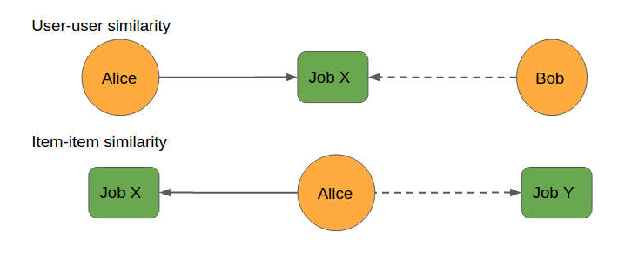
\includegraphics[scale=0.85]{CF.pdf}\\
  \caption{Common notions of homophily leveraged in collaborative filtering }\label{1}
\end{figure}


\begin{enumerate}
  \item \textbf{User-User Similarity:} Let us assume there are two job-seekers, Alice and Bob, who have similar educational qualification and similar experience and live in the same region. Now if one of them, say Alice, applies for a job $X$, then it is highly likely that Bob will also apply for the same job.
  \item \textbf{Item-Item Similarity:} On the other hand, let us assume there is a job item $Y$ that is similar to $X$ in terms of job title, location, experience and background requirements. If Alice applies for the job $X$, then it is quite likely that Alice will also apply for job $Y$.
\end{enumerate}
There are some challenges with this approach.
\begin{enumerate}
  \item \textbf{Sparsity:} As the interaction dataset is very sparse, there are fewer facts than the inferences to be made.
  \item \textbf{Definition of Similarity:} There should be a concrete definition of similarity. The similarity should not be computationally expensive given the huge amount of data that we are dealing with.
  \item \textbf{Gray/Black Sheep Behavior} The actual behaviors of some users are very different from others who are otherwise similar in their meta-information. For example, even though two students did their MS in Computer Science with focus on recommendation systems, one might want to pursue something extremely different in career, e.g. Music. Such gray/black sheep behavior cannot be captured by collaborative filtering approaches.
\end{enumerate}
%It is anyway difficult to identify such users, and provide them with quality recommendations unless the system explicitly asks for such details. As our data do not have any such explicit information, we have not yet found any way to deal with this issue.

We try to address the second challenge mentioned above. Essentially, we want to answer whether the two users or two items are similar or not. For this we considered two approaches.
\begin{enumerate}
  \item \textbf{K-Means Clustering:} We run $K$-Means clustering on users and items dataset. The users (or items) belonging to the same cluster are considered as similar and the ones in different clusters are considered to be dissimilar. The drawback of this approach is that the quality depends on the number of clusters that need to be chosen manually.
  \item \textbf{Cosine Similarity:} The similarity, $S$, of two entities are quantified by the dot product of the corresponding feature vectors normalized by the length of the vectors as shown in equation 1. $U_x$ and $I_y$ represent the feature vectors of user $x$ and item $y$.
      \begin{equation}\label{1}
        S(U_i, U_j) = \frac{U_iU_j}{|U_i||U_j|}; S(I_i, I_j) = \frac{I_iI_j}{|I_i||I_j|}
        \end{equation}
      The potential drawback is that it is not scalable. We have over a million users and a million items. To generate recommendations for a particular user using user-user similarity, we will have to scan through all other users and find similarities. This would mean an intractable computational overhead.
\end{enumerate}

To circumvent their individual drawbacks, we combined the two. We first divided the users and items into clusters. When generating recommendations for a user, we consider only the users belonging to the same cluster and weigh their contributions according to the cosine similarity. If two users are in the same cluster, their similarity is computed as the cosine similarity of the respective feature vectors. On the other hand, users belonging to different clusters are assumed to have similarity $0$. Therefore, the effective similarity calculation is cosine similarity, but the computational overhead is greatly reduced by using $K$-Means clustering.

Suppose, for example, we want to estimate how the user $u$ will interact with item $i$ if it is shown to them. This is just another way of saying that we want to populate the interaction matrix and we want to find an appropriate interaction value. As shown in equation $2$, we can impute the interaction of user $u$ with item $i$ with the average of interactions of other users $v$, in the same cluster $C_u$, with item $i$ weighted by cosine similarities of $u$ with them.
\begin{equation}\label{2}
    I(u, i) = \frac{\sum_{v \in C_u}S(u, v)I(v, i)}{\sum_{v \in C_u}S(u, v)}
\end{equation}
Or, we can impute it with the average of interactions of user $u$ with other items $j$ in same cluster $C_i$ as the item $i$, weighted by their cosine similarities with item $i$.
\begin{equation}\label{3}
    I(u, i) = \frac{\sum_{j \in C_i}S(i, j)I(u, j)}{\sum_{j \in C_i}S(i, j)}
\end{equation}

Please note that the feature vectors used in K-Means clustering and finding cosine similarity are generated by 1-hot encoding the features present in raw users and items datasets. This results in $108$ features in users data and $87$ features in items data. Some features like job roles and tags were not included; these would make the feature set huge.

\subsection{Scoring}
So far we have considered only impression and interaction datasets, and have tried to find implicit relations between users and items. But we also have separate datasets for users and items, and using the fields in those datasets, we can find if a user is likely to apply for a job or not. For overall ranking, we plan to use the user and job description information for ranking in combination with the impression and interaction datasets.

The high level idea is that for generating recommendations to a user, we can assign scores to each item, and then rank those items according to the score. The score consists of the frequency of the item shown to the user -- this can be obtained from the impression dataset. If there has been a positive interaction in past, we can include that interaction as well. For a user to apply for a job, there should be some overlap in the items job roles and users current job roles. There are some other components of the score as well, such as whether career level, industry and discipline of users and jobs match. All these components are weighted differently. The scoring function looks like equation $4$.
\begin{multline}\label{}
    Score = w_1 (\mbox{impression frequency}) + w_2 (\mbox{Interaction score})\\
            + w_3 (\mbox{no. of overlaps in user job-roles and item-titles})\\
            + w_4 (I[\mbox{career level match}])
            + w_5 (I[\mbox{discipline IDs match}]) \\
            + w_6 (I[\mbox{industry IDs match}]
            + w_7 (I[\mbox{regions match}])
\end{multline}

We followed two approaches to assign weights $w_i, \forall i \in \{1, 2, \ldots, 7\}$.
\begin{enumerate}
  \item \textbf{Heuristic Scoring:} Based on our understanding of data developed in previous sections, we assigned weights heuristically. The weights were: $w_1=1 , w_2=100, w_3=10, w_4=12, w_5=10, w_6=5,$ and $w_7=2$. As we will see in Section $4$, this produced a lightweight and fairly strong recommendation system.
  \item \textbf{Linear Regression:} We also set up a linear regression problem in order to learn these weights. For regression, each user-item pair is considered as a data point. Features include: number of items overlap in job roles, career level match, discipline match, industry match and region match, as shown in equation $4$. As shown in Section $4$, this does provide significant improvement over the heuristic approach.
\end{enumerate}

\subsection{Gradient Boosting}
To further improve our results, we applied gradient boosting method. We describe below the process in detail.

\subsubsection{Extended Feature Set}
In addition to the features of linear regressions, we  included the actual individual user and item meta information, and the previous interaction the user had had with the item. This yielded over $200$ features. The job items with which the user had no interaction in past were assigned the previous interaction score of $0$.

\subsubsection{Missing Value Imputation} Some of the features in user dataset, for example career level, had lot of missing or unknown values. In order to better utilize the data, we imputed those missing values. For this, we trained Random Forest with $100$ trees on a random sample of $10,000$ observations with non-missing fields, and used the trained random forest to predict the missing features.

\subsubsection{Training Process} We used caret [4] and AppliedPredictiveModeling [5] libraries in $R$ to train our model to predict what interaction a user will have with an item. We ran $5$-fold cross-validation; in each fold the data is randomly split into $80:20$ ratio for training and validation purposes, respectively. Due to computational overhead, we trained models on different subsets of data with $300K$ observations, and chose the best among them. The attributes of the best model are mentioned in Table 1.

\begin{table}
\centering
\caption{Attributes of the Gradient Boosting Model}
\begin{tabular}{|c|l|} \hline
Attribute &  Value \\ \hline
Number of Trees &  500 \\ \hline
Shrinkage & 0.1 \\ \hline
Interaction depth & 7\\ \hline
Min observation in Terminal node  & 10\\ \hline
Root mean square error & 0.46\\
\hline\end{tabular}
\end{table}

 %The best model consist of $500$ trees with shrinkage of $0.1$, interaction depth of $7$ and n.minobsinnode (minimum observation in terminal node) of $10$. The Root Mean Square Error (RMSE) of the model was $0.46$.


\section{Experiments}
Using different approaches mentioned in the previous section, we obtained top $30$ job recommendations for each of the $150K$ test users. The result were submitted to the competition website. The website processed the output file and returned a score representing the effectiveness of the recommendation system.

\subsection{Evaluation Criteria}
The evaluation score used by the competition is shown on [2]. The overall score is the sum of the scores obtained for individual test users. The score for a particular test user is the combination of recall, precision at various positions and a function called \emph{userSuccess}$(r, t)$. For each user, there exists a two ordered list of items: $T$, the ground truth of the items that the user actually interacted with, and $S$, the list uploaded by us. \emph{userSuccess} returns $1$ if at least one relevant job was returned for a given user else returns $0$. The precision and recalled are defines as equation 5.

\begin{eqnarray}
\nonumber
  \mbox{precision@k} = \frac{\mbox{$\#$ items (among top k) the user clicked}}{k} \\
 \mbox{recall} = \frac{\mbox{$\#$ items (among top $30$) the user clicked}}{\mbox{total $\#$ items the user clicked}}
\end{eqnarray}

\subsection{Performance Evaluation}
The scores obtained from our submissions are shown in Table 2. Please note that the ranks mentioned in the table are according to the current official public leader board. The ranks at time of submission were different. For gradient boosting model, the score and rank were obtained from unofficial leader-board.

It can be seen that our initial models, which mostly deal only with the explicit information given in the interactions and impressions datasets, perform reasonably well given their simplicity. Although collaborative filtering approaches are common in recommendations systems, we see that these do not perform very well in our problem setup. The reason being the sparsity and high-dimensionality of our datasets.

The more advanced models that we have developed represent strong recommendation systems. These perform really well in the competition. Our insightful heuristic scoring mechanism is ``lightweight" and beats majority of submissions. Its simplicity can be vital in quick deployment. This heuristic scoring model, in which we are using all the available datasets, is well augmented by linear regression model. In this, rather than assigning weights according to our understanding of user-behavior, we learn the importance of the features through training on the data. It is worth being noted that learning the weights from data does increase the score by a significant amount.

Finally, to exploit the non-linear relations the features may have with the interaction value, and to use both categorical and numerical features, we took gradient boosting that is a decision tree based ensemble approach. Although trained on very small subsets of full data, it beats the linear model by good margin. Our final model is ranked \textbf{20th} on both official and unofficial leader-boards.

\begin{table}
\centering
\caption{Performance Scores of Various Approaches}
\begin{tabular}{|c|c|l|} \hline
Approach &  Score       & Rank  \\ \hline
Baseline &  26,857.38   & 100 \\ \hline
User User similarity & 85,491.27  & 81 \\ \hline
Interactions & 180,112.15 & 72\\ \hline
Impressions  & 279,062.28 & 48\\ \hline
Heuristic Scoring & 456,487.86 & 23\\ \hline
Linear Regression & 468,767.08 & 20 \\ \hline
\textbf{Gradient Boosting} & \textbf{473,758.10} & \textbf{20}\\
\hline\end{tabular}
\end{table}

\section{Conclusions}
In this paper, we presented our work to build a job recommendation system for XING as a part of ACM RecSys 2016 challenge.
We took a bottom-up approach and first analyzed how individual datasets can help us build a strong recommendation system.
After deeply studying the data and getting useful insights, we played with a lot of heuristics, and we were able to build a well performing ``lightweight" recommendation system. In order to improve the performance of our system, we applied linear regression and gradient boosting methods. Missing values were imputed using Random Forests. These more sophisticated methods indeed improved the results. Our team, ``Falcon", was ranked \textbf{20th} on the official leader-board of the competition.

\section{Future Work}
We can do some user behavior analysis using temporal information that we have in our impression and interactions datasets. This involves understanding a user's session through temporal analysis. For example, given a user with a few interaction data points we can predict their next interaction in the current session.

\begin{thebibliography}{1}
\bibitem{1}
RecSys Challenge 2016 Official Website. \emph{Available at}: \url{http://2016.recsyschallenge.com/}

\bibitem{2}
RecSys Challenge 2016 GitHub. \emph{Available at}: \url{https://github.com/recsyschallenge/2016}
%B. Sarwar, G. Karypis, J. Konstan and J. Riedl. Application of dimensionality reduction in recommender system-a case study. \emph{Technical Report No. TR-00-043}, 2003. Minnesota Univ Minneapolis Dept of Computer Science.

\bibitem{3}
J. B. Schafer, D. Frankowski, J. Herlocker and S. Sen. Collaborative filtering recommender systems. \emph{In The adaptive web} 2007, pp. 291-324. Springer Berlin Heidelberg.

\bibitem{4}
\begin{sloppypar}
Caret: classification and regression training. \emph{Available at}: \url{https://cran.r-project.org/web/packages/caret/index.html}
\end{sloppypar}

\bibitem{5}
AppliedPredictiveModeling: Functions and Data Sets for `Applied Predictive Modeling'. \emph{Available at}: \url{https://cran.r-project.org/web/packages/AppliedPredictiveModeling/index.html}

\end{thebibliography}

\end{document}
